Sha-3 ist eine vom US-amerikanischen "National Institute of Standards and Technology" definierte Familie von kryptographischen Hashfunktion.
Bei einer kryptographischen Hashfunktion handelt es sich um eine Funktion, die zu einer Eingabe beliebiger Länge eine Art Prüfsumme fixer Länge berechnet, den sogenannten Hash.
Dieser Hash dient als eine Art Fingerabdruck. Damit eine solche Hashfunktion als kryptographisch sicher gilt, soll es nicht effizient möglich die Funktion umzukehren.
Generell erwartet man folgende grundlegende Eigenschaften von solchen Hashfunktionen $H$:
\begin{enumerate}
	\item Schwache Kollisionsresistenz: Zu einer gegebenen Nachricht $M$ soll es praktisch unmöglich sein eine zweite Nachricht $M^\prime$ zu finden, die den gleichen Hash besitzt, also $H(M) = H(M^\prime)$
	\item Starke Kollisionsresistenz: Es soll praktisch unmöglich sein zwei Nachrichten $M$ und $M^\prime$ zu finden, die den selben Hashwert gesitzen, also $H(M) = H(M^\prime)$
\end{enumerate}
Bei der Frage, was als "praktisch unmöglich" zählt, betrachtet man typischerweise eine ganze Familie an Hashfunktionen $\mathbb{H}$ mit einem auswählbaren Sicherheitsparameter $n$ und verlangt,
dass es keine probabilistische Turingmaschine gibt, die das entsprechende Problem mit einer Wahrscheinlichkeit $p>\frac{2}{3}$ in einer Laufzeit polynomiell in $n$ löst.
Das Problem liegt also außerhalb der Komplexitätsklasse $BPP$. Analog definiert man auch die Resistenz gegen Quanten-Angriffe, indem man verlangt, dass das Problem auch außerhalb der Komplexitätsklasse BQP liegt.

Um Anfragen beliebiger Länge bearbeiten zu können, bestehen Hashfunktionen typischerweise aus drei Teilen. Mit Hilfe einer \textbf{Padding}-Funktion wird die Eingabe so erweitert,
dass die Länge ein ganzzahliges Vielfaches einer von der Hashfunktion benötigten Blocklänge ergibt. Die Eingabe kann so in mehrere gleich große Blöcke eingeteilt werden.
Aus einer \textbf{Kompressionsfuntion} oder wie im Fall von SHA-3 einer \textbf{Permutation} wird dann eine Funktion konstruiert,
die nacheinander die Blöcke mit dem Ergebnis der Permutation kombiniert und weiterverarbeitet. Während viele bekannte Hashfunktionen dazu die Merkle-Damg\r{a}rd-Konstruktion,
verwendet SHA-3 die sogenannte \textbf{Schwammkonstruktion}. Wie diese genau aussieht und wie sie funktioniert, werden wir später in Abschnitt \ref{sec:schwammkonstruktion} sehen.

Dazu wird die Eingabe mithilfe eines \textbf{Paddings} in mehere gleich große Blöcke aufgeteilt. Die Blöcke werden nacheinander über eine \textbf{Schwammkonstruktion}
zu einem 1600 Bit breiten Bitvektor kombiniert, woraus dann der endgültige Hash ausgelesen wird. Neben den vier Kandidaten, die in Tabelle \ref{tab:uebersicht_sha3} dargestellt sind,
gibt es außerdem noch die beiden Funktionen $SHAKE128$ und $SHAKE256$, bei denen sich die Ausgabegröße beliebig festlegen lässt.
Sie unterscheiden sich in ihrer Funktionsweise nicht wesentlich von den anderen Funktionen, weshalb wir sie hier nicht weiter beachten werden.
\begin{table}
	\centering
	\begin{tabular}{lrrr}
		Name & Kapazität $c$ & Blocklänge $r$ & Hash-Länge \\
		\hline
		SHA3-224 & 448 Bit & 1152 Bit & 224 Bit \\
		SHA3-256 & 512 Bit & 1088 Bit & 256 Bit \\
		SHA3-384 & 768 Bit & 832 Bit & 384 Bit \\
		SHA3-512 & 1024 Bit & 576 Bit & 512 Bit
	\end{tabular}
	\caption{Übersicht über die verschiedenen SHA-3 Hashfunktionen}
	\label{tab:uebersicht_sha3}
\end{table}

\newcommand{\bigcomp}{%
  \DOTSB
  \mathop{\vphantom{\sum}\mathpalette\bigcomp@\relax}%
  \slimits@
}
\newcommand{\bigcomp@}[2]{%
  \begingroup\m@th
  \sbox\z@{$#1\sum$}%
  \setlength{\unitlength}{0.9\dimexpr\ht\z@+\dp\z@}%
  \vcenter{\hbox{%
    \begin{picture}(1,1)
    \bigcomp@linethickness{#1}
    \put(0.5,0.5){\circle{1}}
    \end{picture}%
  }}%
  \endgroup
}
\newcommand{\bigcomp@linethickness}[1]{%
  \linethickness{%
      \ifx#1\displaystyle 2\fontdimen8\textfont\else
      \ifx#1\textstyle 1.65\fontdimen8\textfont\else
      \ifx#1\scriptstyle 1.65\fontdimen8\scriptfont\else
      1.65\fontdimen8\scriptscriptfont\fi\fi\fi 3
  }%
}

\section{Keccak-Permutation}
Als Grundlage für alle SHA3-Funktionen dient eine Instanz der Keccak-Permutationsfamilie KECCAK-f.
Für eine kryptographische Sicherheitsanalyse betrachtet man in der Regel das asymptotische Verhalten der erwarteten Laufzeit eines Angreifers.
Hierzu benötigt man eine Funktion mit variablem Sicherheitsparameter, damit diese Analyse durchgeführt werden kann.
Wir interessieren uns hier allerdings nur für die konkrete Instanz mit einem festen Sicherheitsparameter, die vom SHA-3 Standard \comment{(Cite missing, [2])} festgelegt wird.
Die genaue Definition mit variablem Sicherheitsparameter ist zum Nachlesen auch in \comment{(Cite missing, [2])} angegeben.
Wir wollen uns nun zuerst einmal den Zustandsvektor, auf dem die Permutation arbeitet, ein wenig genauer anschauen,
bevor wir uns die fünf Unterfunktionen ansehen, aus denen die KECCAK-f Permutation aufgebaut ist.

\subsection{Zustandsvektor}
Die KECCAK-f Permutation arbeitet auf einem 1600 Bit breiten Zustandsvektor, auch \textbf{State Array} genannt.
Am besten lässt er sich als dreidimensionale Struktur der Form 5x5x64 Bit vorstellen, siehe Abb. \ref{fig:statearray}.
Wir indizieren ein solches State Array \textbf{A}[x][y][z] über $x,y \in \{0,...,4\};\ z \in \{0,...,63\}$. Außerdem nennen wird
\begin{align*}
	&Lane(\textbf{A},x,y) \coloneq \textbf{A}[x][y] && \coloneq \textbf{A}[x][y][0] \mathbin\Vert ... \mathbin\Vert \textbf{A}[x][y][63] && \text{ eine \textbf{Lane} von \textbf{A},} \\
	&Zeile(\textbf{A},y,z) && \coloneq \textbf{A}[0][y][z] \mathbin\Vert ... \mathbin\Vert \textbf{A}[4][y][z] && \text{ eine \textbf{Zeile} von \textbf{A},} \\
	&Spalte(\textbf{A},x,z) && \coloneq \textbf{A}[x][0][z] \mathbin\Vert ... \mathbin\Vert \textbf{A}[x][4][z] && \text{ eine \textbf{Spalte} von \textbf{A},} \\
	&Slice(\textbf{A},z) && \coloneq Zeile(\textbf{A},0,z) \mathbin\Vert ... \mathbin\Vert Zeile(\textbf{A},4,z) && \text{ einen \textbf{Slice} von \textbf{A}.} \\
\end{align*}
\begin{figure}
	\center
	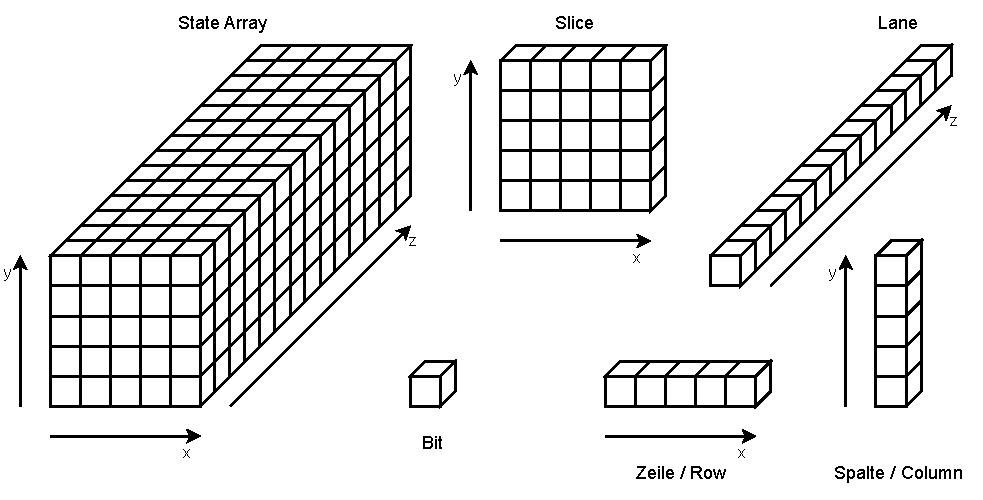
\includegraphics{images/StateArrayBeschreibung.pdf}
	\caption{Blockrepräsentation des State Array}
	\label{fig:statearray}
\end{figure}
Die Konvertierung eines eindimensionalen Bitvektors \textbf{V} in dieses dreidimensionale State Array \textbf{A} funktioniert wie folgt:
\begin{align*}
	\textbf{A}[x][y][z] \coloneq \textbf{V}[64(5y + x) + z] & \forall x,y = 0,...,4; z = 0,...,63
\end{align*}
Die Lanes werden also der Reihe nach erst in x-Richtung und dann in y-Richtung mit dem Inhalt von \textbf{V} gefüllt.

\subsection{Unterfunktionen}
\label{cha:sha3_unterfunktionen}

\subsubsection{Theta-Unterfunktion}
\begin{figure}
    \center
    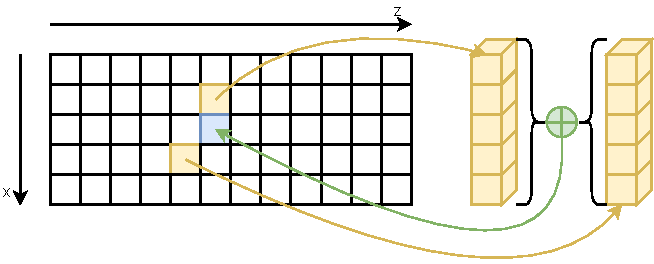
\includegraphics{images/theta.pdf}
    \caption{Spaltensummierung der $\theta$-Funktion}
    \label{fig:definition_theta}
\end{figure}
Die erste Unterfunktion der Keccak-Permutation ist Theta ($\theta$). Sie modifiziert jedes Bit eines State Arrays, indem sie zwei benachbarte Spalten auf das Bit aufsummiert, siehe Abb. \ref{fig:definition_theta}.
\begin{align*}
    \theta (\textbf{A}) & \coloneq \textbf{A}^\prime \text{ mit } \\
    \textbf{C}[x] & \coloneq \textbf{A}[x][0] \oplus ... \oplus \textbf{A}[x][4] && \forall x = 0,...,4 \\
    \textbf{D}[x] & \coloneq \textbf{C}[(x - 1) mod\ 5] \oplus rotr(C[(x + 1) mod\ 5], 1)\ && \forall x = 0,...,4 \\
    \textbf{A}^\prime[x][y] & \coloneq \textbf{A}[x][y] \oplus \textbf{D}[x]\ && \forall x = 0,...,4;\ y = 0,...,4
\end{align*}
Man beachte, dass hier die State Arrays nur mit x und y indiziert werden, alle Operationen finden also immer auf ganzen Lanes gleichzeitig statt.
Ein 64-Bit Prozessor kann also Theta mit Hilfe von ein paar bitweisen XOR-Operationen auf 64-Bit Operanden berechnen.
\textbf{C} dient hierzu als Zwischenspeicher für Spaltensummen und \textbf{D} wird verwendet, um jeweils zwei Spaltensummen aufzuaddieren.

\subsubsection{Rho-Unterfunktion}
\begin{figure}
    \center
    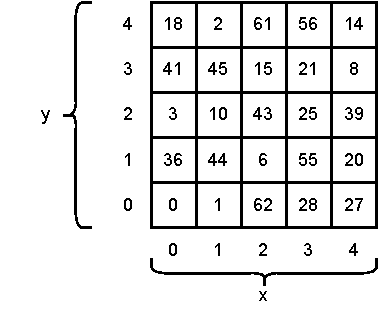
\includegraphics{images/rho.pdf}
    \caption{Rotationsdistanzen der Lanes für $\rho$}
    \label{fig:definition_rho}
\end{figure}
Bei der Rho-Unterfunktion ($\rho$) handelt es sich um eine einfache Bitrotation der einzelnen Lanes.
Bis auf die Lane bei $x=0 und y=0$ werden alle Lanes um eine konstante Distanz nach links rotiert.
Die genauen Distanzen sind in Abb. \ref{fig:definition_rho} aufgeführt.
\begin{align*}
    \rho (\textbf{A}) & \coloneq \textbf{A}^\prime \text{ mit } \\
    \textbf{A}^\prime[x][y] & \coloneq rotl(\textbf{A}[x][y], d[x][y])\ \forall x = 0,...,4;\ y = 0,...,4 \\
    d & :\text{ Eine 5x5 Matrix an Konstanten, siehe Abb. \ref{fig:definition_rho}}
\end{align*}

\subsubsection{Pi-Unterfunktion}
\begin{figure}
    \center
    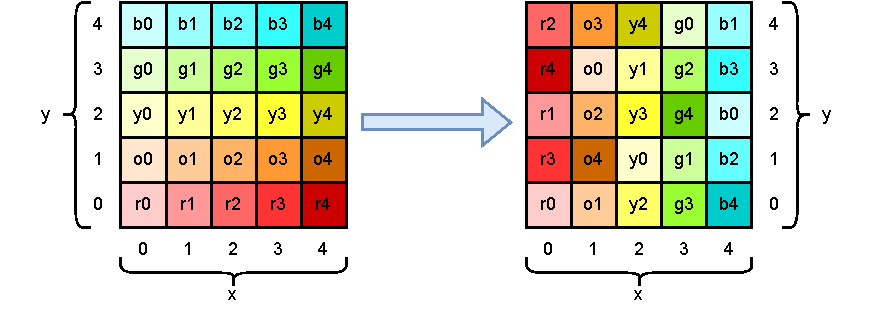
\includegraphics{images/pi.pdf}
    \caption{Visualisierung der $pi$-Permutation}
    \label{fig:definition_pi}
\end{figure}
Die Pi-Unterfunktion ($\pi$) permutiert die Lanes eines State Arrays untereinander nach einer einfachen Vorschrift.
Dass diese Abbilung injektiv ist, folgt direkt aus der Nullteilerfreiheit des Rings $\mathbb{Z}/5\mathbb{Z}$,
oder man akzeptiert einfach die Veranschaulichung in Abb. \ref{fig:definition_pi}.
\begin{align*}
    \pi (\textbf{A}) & \coloneq \textbf{A}^\prime \text{ mit } \\
    \textbf{A}^\prime[x][y] & \coloneq \textbf{A}[(x + 3y)\ mod\ 5][x]\ \forall x = 0,...,4;\ y = 0,...,4
\end{align*}

\subsubsection{Chi-Unterfunktion}
Im Gegensatz zu allen anderen Unterfunktionen ist Chi ($\chi$) nicht affin-linear.
Interessanterweise ist sie trotzdem invertierbar, solange die Anzahl an Spalten ungerade ist \comment{(Cite Missing, [1])}, in unserem Fall fünf. 
Das bedeutet, dass die Keccak-p Rundenfunktion sowie die Keccak-p Permutation invertierbar ist.
Trotzdem eignet sie sich wie wir sehen werden um eine sichere Hashfunktion zu konstruieren,
da die Art und Weise wie sie verwendet wird die Nicht-Invertierbarkeit nicht benötigt.
\begin{align*}
    \chi (\textbf{A}) & \coloneq \textbf{A}^\prime \text{ mit } \\
    \textbf{A}^\prime[x][y] & \coloneq \textbf{A}[x][y] \oplus ((\sim \textbf{A}[(x + 1)\ mod\ 5][y]) * \textbf{A}[(x + 2)\ mod\ 5][y])\ & \forall x = & 0,...,4;\\
    && y = & 0,...,4
\end{align*}

\subsubsection{Iota-Unterfunktion}
\begin{table}
	\centering
	\begin{tabular}{rrrr}
		Rundenindex $r$ & Rundenkonstante $C[r]$ & Rundenindex $r$ & Rundenkonstante $C[r]$\\
		\hline
		 0 & 0x1 &
		 1 & 0x8082\\
		 2 & 0x800000000000808a &
		 3 & 0x8000000080008000\\
		 4 & 0x808b &
		 5 & 0x80000001\\
		 6 & 0x8000000080008081 &
		 7 & 0x8000000000008009\\
		 8 & 0x8a &
		 9 & 0x88\\
		10 & 0x80008009 &
		11 & 0x8000000a\\
		12 & 0x8000808b &
		13 & 0x800000000000008b\\
		14 & 0x8000000000008089 &
		15 & 0x8000000000008003\\
		16 & 0x8000000000008002 &
		17 & 0x8000000000000080\\
		18 & 0x800a &
		19 & 0x800000008000000a\\
		20 & 0x8000000080008081 &
		21 & 0x8000000000008080\\
		22 & 0x80000001 &
		23 & 0x8000000080008008
	\end{tabular}
	\caption{$\iota$-Rundenkonstanten für die einzelnen Runden der Keccak-f Permutation}
	\label{tab:rundenkonstanten}
\end{table}
Die letzte Unterfunktion Iota ($\iota$) modifiziert lediglich die Lane an Position (x,y) = (0,0), indem sie sie mit einer Rundenkonstante per XOR kombiniert.
Die genauen Werte der Rundenkonstanten C[r] sind in Tabelle \ref{tab:rundenkonstanten} dargestellt.
Damit wir nachher die Rundenfunktion besser darstellen können, definieren wir neben der zweistelligen Funktion
$\iota (\textbf{A}, r)$ noch die über dem Rundenindex $r$ parametrisierte Funktion $\iota_r (\textbf{A})$.
\begin{align*}
    \iota (\textbf{A}, r) & \coloneq \textbf{A}^\prime \text{ mit } \\
    \textbf{A}^\prime[x][y] & \coloneq
    \begin{cases}
        \textbf{A}[x][y] \oplus C[r], & x = 0 \text{ und } y = 0 \\
        \textbf{A}[x][y], & \text{sonst}
    \end{cases} \\
    \iota_r (\textbf{A}) & \coloneq \iota(\textbf{A}, r)
\end{align*}



\subsection{KECCAK-p}
Die fünf Unterfunktionen werden zur Rundenfunktion $Rnd_r$ kombiniert, mit der dann die Permutationsfunktion KECCAK-p definiert wird:
\begin{align*}
	Rnd_r(\textbf{A}) & \coloneq (\iota_r \circ \chi \circ \pi \circ \rho \circ \theta)(\textbf{A})\ \forall r \in \{0,...,23\}
    \text{KECCAK-p} (\textbf{A}) & \coloneq (\bigcomp_{i = 0}^{23} Rnd_i)(\textbf{A}) \\
\end{align*}

\subsection{KECCAK-f}
Für die letztendliche Permutation wird die Rundenfunktion KECCAK-p mehrfach hintereinander angewendet.
Wir definieren hier allerdings nur die eine Instanz der gesamten KECCAK-f Familie, die wir am Ende für die SHA-3 Hashfunktionen benötigen.
Die vollständige Definition der Familie ist in \comment{(Cite Missing, [2])} 
\begin{align*}
    \text{KECCAK-f} (\textbf{A}) \coloneq (\bigcomp_{i = 0}^{23} \text{KECCAK-p}_{i})(\textbf{A})
\end{align*}

\section{Padding-Funktion $pad10^*1$}
Um eine Eingabe beliebiger Länge gescheit verarbeiten zu können, wird eine Padding-Funktion verwendet.
Diese nimmt eine Eingabe beliebiger Länge entgegen und erzeugt ein einfaches dynamisches Datenmuster,
sodass, wenn man es an die Eingabe anhängt, das Ganze eine länge hat, die ein Vielfaches der gewünschten Blocklänge ist.
SHA-3 verwendet als Padding die Funktion $pad10^*1$. Diese erzeugt, wie der Name schon vermuten lässt,
einen Bitvektor, der bis auf das erste und letzte Bit nur aus Nullen besteht.
\begin{align*}
	&\begin{alignedat}[t]{2}
	\text{Für} & \text{ eine Eingabe } & M & \in \{0,1\}^*, \\
	& \text{ eine verlangte Blocklänge } & r & \in \mathbb{N} \\
	\end{alignedat} \\
	& \text{ist } pad10^*1(r, M) \coloneq 1 \mathbin\Vert 0^{(-|M| - 2) mod\ r} \mathbin\Vert 1
\end{align*}

\section{Schwammkonstruktion}
	\label{sec:schwammkonstruktion}
	\begin{figure}
		\center
		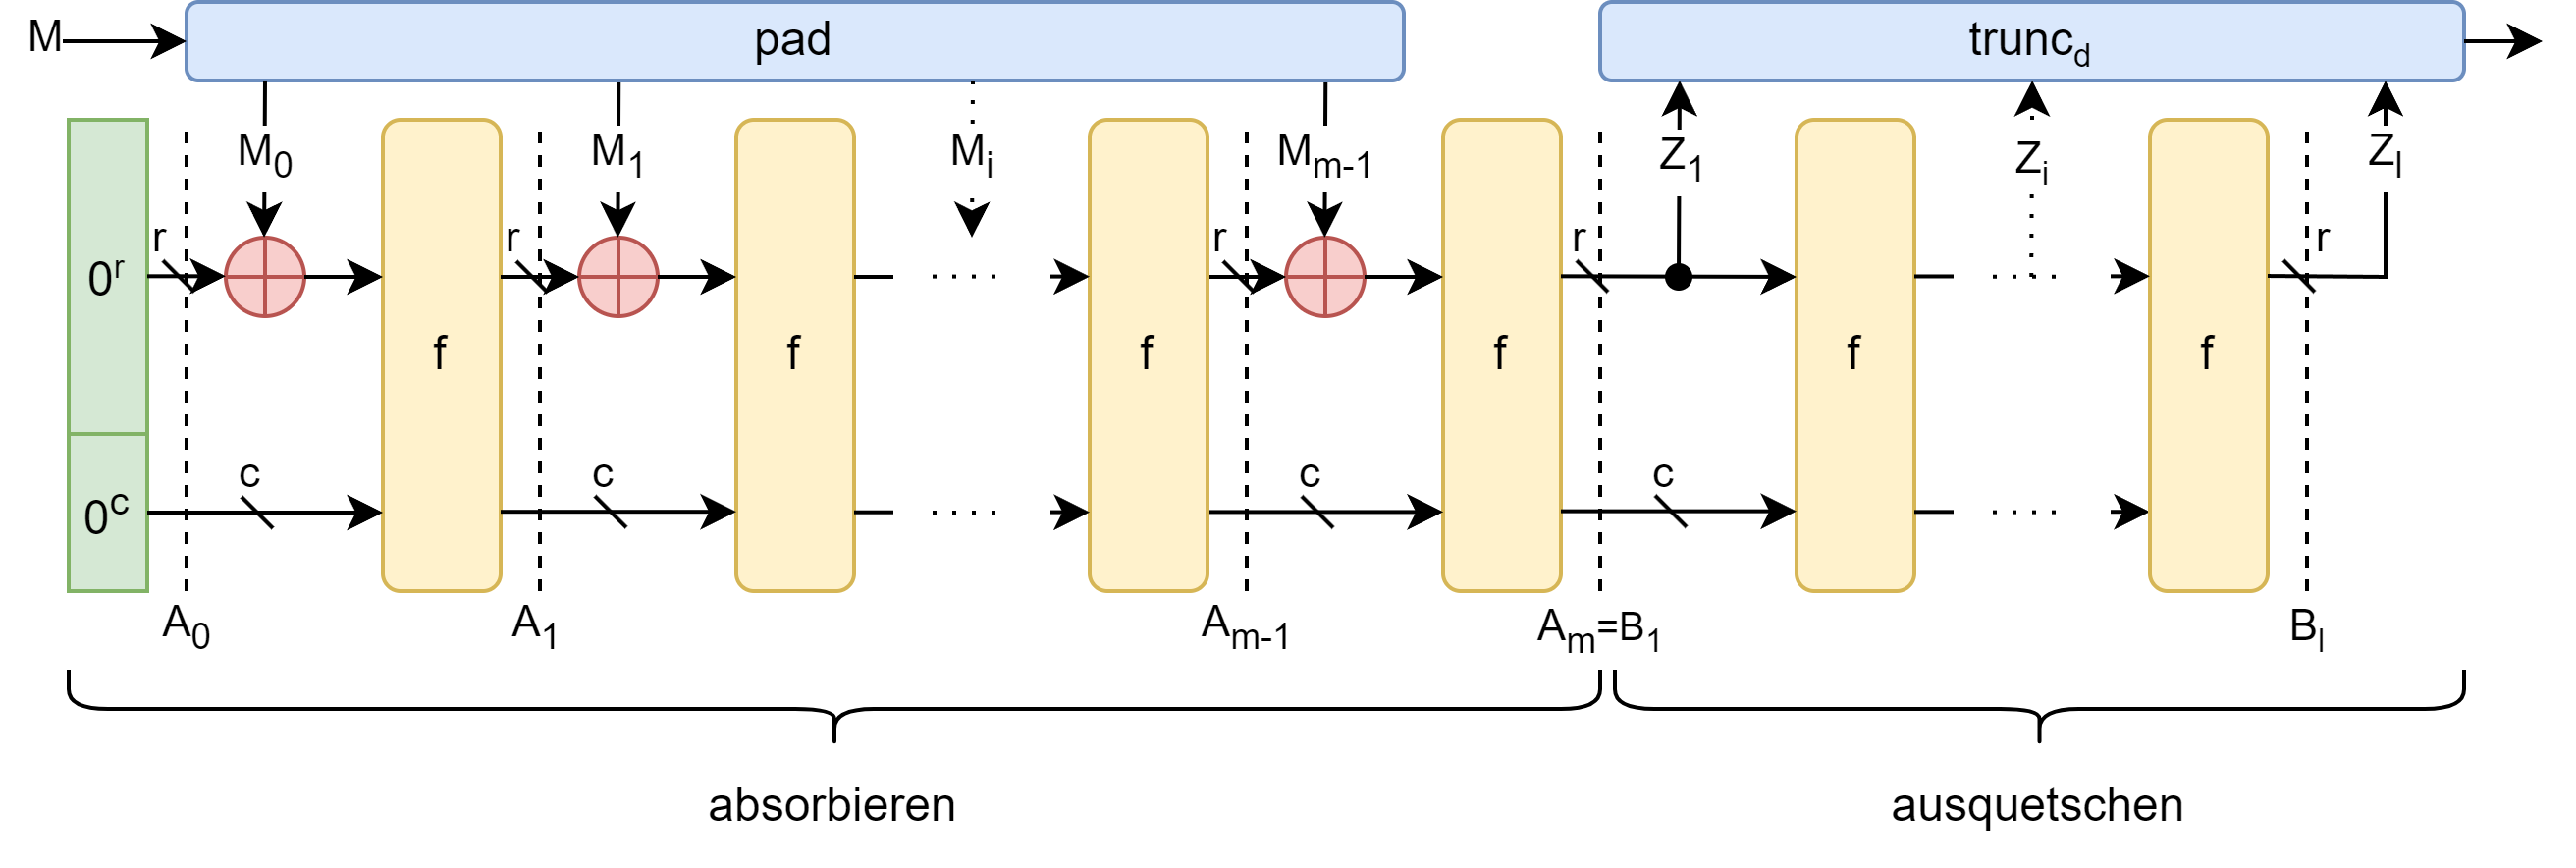
\includegraphics[scale=0.175]{images/Schwammkonstruktion.png}
		\caption{Aufbau der Schwammkonstruktion [Cite missing]}
		\label{fig:schwammkonstruktion}
	\end{figure}
	Um beliebig lange Eingaben zu einem kurzten Hashwert komprimieren zu können, verwendet SHA-3 die sogenannte Schwammkonstruktion.
	Sie erlaubt es eine Eingabe beliebiger Länge auf eine Ausgabe einer beliebigen anderen Länge d abzubilden.
	Dazu wird die Eingabe, wie in Abb \ref{fig:schwammkonstruktion} veranschaulicht, erst mit Hilfe einer Padding-Funktion in mehrere gleich große Blöcke einer festgelegten Länge abgebildet.
	Die Eingabeblöcke werden dann der Reihe nach vom Schwamm "absorbiert". Danach werden auf ähnliche Weise die Ausgabeblöcke aus dem Schwamm "ausgequetscht".
	Diese Ausgabeblöcke werden dann zur finalen Ausgabe zusammengesetzt. Wenn die Ausgabelänge kein Vielfaches der Blocklänge sein sollte, wird der Rest einfach abgeschnitten.
	Der genaue Definition der Schwammkonstruktion über einer Transformation $f$ mit einer Paddingfunktion $pad$ sieht folgendermaßen aus:
	
	\begin{align*}
		&\begin{alignedat}[t]{2}
			Seien\ & n \in \mathbb{N} && \text{ die Transformationsbreite}, \\
			& c \in \{1,...,n\} && \text{ die Kapazität (Anzahl nicht von Blöcken veränderbarer Bits)}, \\
			& r \in \{1,...,n\} && \text{ die Blocklänge}, \\
			& M \in \{0,1\}^* && \text{ die zu verarbeitende Nachricht}, \\
			& m \in \mathbb{N} && \text{ die Anzahl an Blöcken, in die M eingeteilt wird}, \\
			& d \in \mathbb{N} && \text{ die gewünschte Ausgabe}, \\
			& l \coloneq \lceil \frac{d}{r} \rceil && \text{ die benötigte Blockanzahl an Ausgabe}, \\
			& pad: \mathbb{N}x\{0,1\}^* \to (\{0,1\}^r)^+ && \text{ eine Padding-Funktion}, \\
			& f: \{0,1\}^n \to \{0,1\}^n && \text{ eine Transformation}.
		\end{alignedat} \\
		\\
		&\text{Dann ist die Schwammkonstruktion } SPONGE[f,pad,c](M,d) \text{ definiert als:} \\
		&\begin{alignedat}[t]{3}
			SPONGE[f,pad,c](M, d) & \coloneq \mathbf{Z}[0] \mathbin\Vert ... \mathbin\Vert \mathbf{Z}[d-1]\ mit \\
			r & \coloneq 1600 - c \\
			M_1...M_{m} & \coloneq M \mathbin\Vert pad(r, M) \text{ wobei } |M_i| = r\ \forall i = 1,...,m\\
			\mathbf{A}_0 & \coloneq 0^n \\
			\mathbf{A}_i & \coloneq f(\mathbf{A}_{i-1} \oplus (M_{i-1} \mathbin\Vert 0^c))\ & \forall i = 1,...,m \\
			\mathbf{B}_1 & \coloneq \mathbf{A}_{m} \\
			\mathbf{B}_i & \coloneq f(\mathbf{B}_{i-1})\ & \forall i = 2,...,l \\
			\mathbf{Z}_i & \coloneq \mathbf{B}_i[0] \mathbin\Vert ... \mathbin\Vert \mathbf{B}_i[r-1] \\
			\mathbf{Z} & \coloneq \mathbf{Z}_1 \mathbin\Vert ... \mathbin\Vert \mathbf{Z}_l
		\end{alignedat}
	\end{align*}
	
\subsection{SHA3-Hashfunktionen}
Die in \ref{tab:uebersicht_sha3} genannten Hashfunktionen sind nun Instanzen dieser Schwammkonstruktion:
\begin{align*}
	\text{SHA3-224}(M) & \coloneq SPONGE[\text{KECCAK-p},pad10^*1, 448](M \mathbin\Vert 01, 224), \\
	\text{SHA3-256}(M) & \coloneq SPONGE[\text{KECCAK-p},pad10^*1, 512](M \mathbin\Vert 01, 256), \\
	\text{SHA3-384}(M) & \coloneq SPONGE[\text{KECCAK-p},pad10^*1, 768](M \mathbin\Vert 01, 256), \\
	\text{SHA3-512}(M) & \coloneq SPONGE[\text{KECCAK-p},pad10^*1,1024](M \mathbin\Vert 01, 512)
\end{align*}
Die zwei Extrabits "01", die an die Nachricht angefügt werden,
dienen nur dazu die erzeugten Werte von denen anderer Betriebsmodi der KECCAK-p Permutation zu unterscheiden,
wie beispielsweise den beiden SHAKE-Funktionen.

\section{Sicherheitseigenschaften}
Nun ist erstmal noch überhaupt nicht klar, wieso es sich bei den \comment{oben} definierten Funktionen um eine Einwegfunktion handelt.
Schließlich verwendet sie eine sehr leicht invertierbare Permutation. Dazu wollen wir uns die schwammkonstruktion noch einmal etwas genauer anschauen,
in diesem Fall am Beispiel von SHA3-256, wobei wir nur einen Block hashen \comment{(Abb. )}.
Da für eine gehashte Nachricht $M$ nicht die ganze Ausgabe $Hash \mathbin\Vert Trunc$ bekannt ist, sondern nur $Hash$,
muss um aus $Hash$ eine Nachricht $M^\prime$ berechnen zu können, für die  SHA3-256$(M^\prime) = Hash$ gilt,
Eine Belegung für Trunc gefunden werden, sodass die letzten 512 Bits der Eingabe in die KECCAK-p Funktion alle 0 sind.
Selbst wenn die verwendete Permutation einfach invertierbar ist, folgt daraus also nicht gleich, dass auch die Schwammkonstruktion über der Permutation einfach umkehrbar ist.
Diese Überlegung reicht natürlich noch nicht als Beweis, aber gibt einen intuitiven Einblick in die Schwierigkeit, die dem Problem zugrunde liegt.

\subsection{Sicherheit der Schwammkonstruktion}


\subsection{Kollisionsresistenz}

\subsection{Post-Quantum Sicherheit der Schwammkonstruktion}